\documentclass{easyclass}

\usepackage{todonotes}
\usepackage{mathtools}
\usepackage{cancel}
\usepackage{xfrac}
\usepackage{float}
\usepackage{caption}

\tikzstyle{int}=[draw, fill=blue!20, minimum size=2em]
\tikzstyle{init} = [pin edge={to-,thin,black}]
\tikzstyle{sum} = [draw, fill=blue!20, circle, node distance=1cm]

\begin{document}
\begin{titlepage}
    \university{Politicnico di Milano}
    \courseid{MIDA2}
    \title{Model Identification and Data Analysis \par Part 2}
    \author{Edoardo Morassutto}
    \version{2019 -- 2020}
    \instructor{Instructors: Prof \textsc{Sergio Savaresi}\par
    Ing. \textsc{Stefano Dattilo}}
    \maketitle
\end{titlepage}

\tableofcontents

\input{lectures/template.tex}
\section{Table}

\begin{table}[htp]
    \centering
    \begin{tabular}{r|l|p{10cm}}
        Right &  Left  &  Longlonglonglonglonglonglonglong longlonglonglonglonglonglonglonglonglonglonglonglong longlonglonglonglonglong \\
        Right &  Left  &  Longlonglonglonglonglonglong
        longlonglonglonglonglonglonglong
        longlonglonglong
        longlonglonglonglonglonglonglong
    \end{tabular}
    \caption{This is a caption}
    \label{tab:trans-sym}
\end{table}

\section{List}
This is a List:
\begin{itemize}
    \item \textbf{Bullet 1}: Bullet 1 is bullet 1.
    \item \textbf{Bullet 2}: Bullet 2 is bullet 2.
\end{itemize}

\section{Definition}
\begin{definition}\label{def:def1}
\textbf{DEFINITION NAME}: This is a definition.
\end{definition}

% avoid bad break
\vspace{5cm}

\section{Theorem}
\begin{theo}[THEOREM NAME]{theo:theo1}
This is a theorm. Below are equations.
\begin{align}\label{eq:multi-equations}
    \psi(\bvec{a}) &= A\cdot \bvec{a} + \bvec{t}.\\
    R_x &=  \begin{bmatrix}
            0 & \cos(\theta) & -\sin(\theta)\\
            0 & \sin(\theta) & \cos(\theta)\\
            1 & 0 & 0
         \end{bmatrix},
    R_y =  \begin{bmatrix}
            \cos(\theta) & 0 & -\sin(\theta)\\
            \sin(\theta) & 0 & \cos(\theta)\\
            0 & 1 & 0
         \end{bmatrix},
    R_z =  \begin{bmatrix}
            \cos(\theta) & -\sin(\theta) & 0\\
            \sin(\theta) & \cos(\theta) & 0 \\
            0 & 0 & 1
         \end{bmatrix}
\end{align}
\end{theo}

\begin{lem}[LEMMA NAME]{lem:leml}
This is a lemma
\end{lem}

\begin{prf}[LEMMA NAME]{prf:leml}
This is a proof.
\end{prf}

\section{Tikz Pictures}
\begin{figure}[htp]
    \centering
        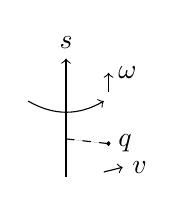
\begin{tikzpicture}[scale=0.6]
            \draw[->] (0,-1)--(0,1.5)node[above] {$s$};
            \draw[->] (-0.8,0.6) to[bend right] (0.8,0.6);
            \draw[->] (0.9, 0.8)--(0.9, 1.2) node[right] {$\omega$};
            \filldraw[dashed] (0,-0.2)--(0.9, -0.3) circle (1pt) node [right] {$q$};
            \draw[->] (0.8, -0.9)--(1.2, -0.8) node[right] {$v$};
        \end{tikzpicture}
    \caption{This is a caption. }
    \label{fig:rotation}
\end{figure}





\curinstructor{Ins Tructor1}

\begin{remark}[Strictly proper systems]
    Notice that for strictly proper systems the delay $k \ge 1$
\end{remark}
\missingfigure{Graphs about strictly proper systems}

\subsection{Representation \#3: convolution of the input with the Impulse Response (IR)}
The third way to represent a system is through the convolution of the input with the \emph{Impulse Response (IR)}.
\missingfigure{Graphs about convolution}
It can be proven that the input-output relationship from $u(t)$ to $y(t)$ can be written as
\[ y(t) = \omega(0) u(t) + \omega(1) u(t-1) + \omega(2) u(t-2) + \cdots \]
It can be rewritten as follows
\[ y(t) = \sum_{k=0}^{\infty} \omega(k) u(t-k) \]
From this, it is clear that $y(t)$ is the convolution of IR with the input signal.
\missingfigure{Block diagram of system}

\section{Transformation between representations}
\missingfigure{Figure of translation between representations}
\subsection{State Space to Transfer function}
Consider a strictly proper system with the following state space representation:
\[
\begin{cases}
    x(t+1) = F x(t) + G u(t)\\
    y(t) = H x(t) + \cancelto{0}{D u(t)}\\
\end{cases}
\Rightarrow
\begin{cases}
    x(t+1) = F x(t) + G u(t)\\
    y(t) = H x(t)\\
\end{cases}
\]
From the system we get
\[ z x(t) = F x(t) + G u(t) \Rightarrow x(t) = (zI - F)^{-1} G u(t) \]
\[ \Rightarrow y(t) = H (zI - F)^{-1} G \cdot u(t) \]
Thus, the transfer function is
\[ W(z) = H(zI - F) ^ {-1} G \]

\begin{example}
\begin{align*}
    F = \begin{bmatrix}
        1 & 0\\
        \frac{1}{2} & 2\\
    \end{bmatrix}
    &&
    G = \begin{bmatrix}
        1\\
        1\\
    \end{bmatrix}
    &&
    H = \begin{bmatrix}
        1 & 0\\
    \end{bmatrix}
    &&
    D = 0
\end{align*}
\begin{align*}
W(z) &=
\begin{bmatrix}
    1 & 0\\
\end{bmatrix}
\left( \begin{bmatrix}
    z & 0\\
    0 & z\\
\end{bmatrix}
-
\begin{bmatrix}
    1 & 0 \\
    \frac{1}{2} & 2\\
\end{bmatrix}\right)^{-1}
\begin{bmatrix}
    1\\
    1\\
\end{bmatrix}
= \begin{bmatrix}
    1 & 0\\
\end{bmatrix}
\begin{bmatrix}
    z-1 & 0\\
    -\frac{1}{2} & z-2\\
\end{bmatrix}^{-1}
\begin{bmatrix}
    1\\
    1\\
\end{bmatrix}\\
&= \begin{bmatrix}
    1 & 0\\
\end{bmatrix}
\frac{1}{(z-1)(z-2)}
\begin{bmatrix}
    z-2 & 0\\
    \frac{1}{2} & z-1\\
\end{bmatrix}
\begin{bmatrix}
    1\\
    1\\
\end{bmatrix}
=
\frac{1}{(z-1)(z-2)}
\begin{bmatrix}
    z-2 & 0\\
\end{bmatrix}
\begin{bmatrix}
    1\\
    1\\
\end{bmatrix}\\
&=
\frac{\cancel{z-2}}{(z-1)\cancel{(z-2)}} = \frac{1}{z-1} = \frac{1}{1-z^{-1}} z^{-1}
\end{align*}
Notice that in this case we only have one pole, but the system is of order two; this comes from the fact that part of the system is non observable.

\end{example}

\subsection{Transfer function to State Space}
This conversion is not very used in practice and it is called the \emph{realization} of a transfer function into a state space model.

Note that the state space representation is not unique, so from a single transfer function we can get infinite different equivalent state space models.

\begin{example}[Control realization]

We assume that the system is strictly proper and that the denominator is monic.
\[ W(z) = \frac{b_0 z^{n-1} + b_1 z^{n-2} + \dots + b_{n-1}}{z^n + a_1 z^{n-1} + a_2 z^{n-2} + \dots + a_n} \]

The formula for the control realization of $W(z)$ is
\begin{align*}
    F = \begin{bmatrix}
        0 & 1 & 0 & \cdots & 0\\
        0& 0 & 1 & \ddots & \vdots \\
        \vdots & \vdots & \ddots & \ddots & 0\\
        0 & 0 & \cdots & 0 & 1\\
        -a_n & -a_{n-1} & \multicolumn{2}{c}{\cdots} & -a_1\\
    \end{bmatrix}
    &&
    G = \begin{bmatrix}
        0\\
        0\\
        0\\
        \vdots\\
        1\\
    \end{bmatrix}
    &&
    H = \begin{bmatrix}
        b_{n-1} & b_{n-2} & \cdots & b_0\\
    \end{bmatrix}
    &&
    D = 0
\end{align*}
\end{example}


%\bibliography{bibfile}

\end{document}
